\pdfinfo{
  /Author {Jonathan Yee}
  /Title {hw5}
  /Keywords{}
}

\newcommand{\courseNum}{10-601 Machine Learning}
%%%%%%%%%% FILL IN THE FOLLOWING INFORMATION %%%%%%%%%%
\newcommand{\recNum}{5}
\newcommand{\recTitle}{Homework 5 - Problem 1}
\newcommand{\hwName}{Jonathan Yee}
\newcommand{\hwAndrewId}{jyee1}
%%%%%%%%%%%%%%%%%%%%%%%%%%%%%%%%%%%%%%%%%%%%%%%%%%%%%%%

\documentclass[11pt]{article}

\usepackage[margin=2.4cm, top=3cm]{geometry}
\usepackage[colorlinks=true]{hyperref}
\usepackage{fancyhdr}
\usepackage{listings}
\usepackage{framed}
\usepackage{mdframed}
\usepackage{multicol}
\usepackage{amsmath, amsfonts, amsthm, amssymb}
\usepackage{enumerate}
\usepackage{graphicx}

\mdfdefinestyle{mybox}{%
rightline=true,innerleftmargin=10,innerrightmargin=10,innertopmargin=5, innerbottommargin=5}

\pagestyle{fancy}

\newenvironment{Section}[1]{
  \vspace{.1in}
  \noindent {\large \bf #1}
}

\newcommand{\mtt}[1]{$\mathtt{#1}$}
\setlength{\parindent}{0in}
\setlength{\parskip}{0.1in}
\renewcommand{\headrulewidth}{0pt}


\newcommand{\realnum}{\mathbb{R}}
\newcommand{\natnum}{\mathbb{N}}
\newcommand{\intnum}{\mathbb{Z}}
\newcommand{\ratnum}{\mathbb{Q}}
\newcommand{\expect}{\mathbf{E}}
\newcommand{\powset}{\mathcal{P}}

% For multicol
%\setlength{\columnsep}{1cm}

\lhead{28 Mar 2015}
\rhead{jyee1, lingzhaj}
\cfoot{\thepage}

\begin{document}

\definecolor{gray}{rgb}{0.5,0.5,0.5}

\lstset{
  basicstyle=\ttfamily,
    language=Java,
    numbers=left,
    numbersep=0.2in,
    xleftmargin=0.75in,
    numberstyle=\ttfamily\color{gray}
}

\begin{Section}{}

\textbf{Data}
\begin{itemize}
	\item 52,152 rows of labeled pixel data
	\item for each given letter, the letter that comes after it, or -1 if none
\end{itemize}

For our project, we see three levels of development: a baseline, and two extensions.

\textbf{Baseline}

We plan to implement two classifiers that we learned in class: Naive Bayes and Logistic Regression.

%\textbf{Naive Bayes}
%
%$y \in \left\{ ``a", ..., ``z" \right\}$. Each label is a letter out of 26 letters.
%$ X = \{ x_1, ..., x_{128} \}, x_i \in \{0,1\} $. Each training sample is a vector of booleans, representing the pixel data.

\textbf{Minor Extension}

Represent each word as a HMM, like below.

\begin{center}
	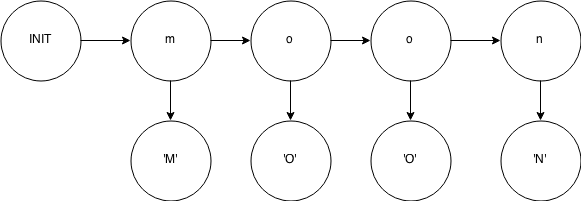
\includegraphics[scale=0.75]{ml_project_hmm.png}
\end{center}
\end{Section}

Each hidden state is a \textbf{letter}. Each observed state is a \textbf{pixel vector}. We need to find the following parameters:
\begin{itemize}
	\item $\phi_{i,j}$ : transition probability from state $i$ to $j$
	\item $\theta_{i}(X)$ : emission probability associated with state $i$ of a pixel vector $X$
\end{itemize}

We plan to use MLE to find $\phi_{i,j}$. Let $c_1, c_2$ be consecutive letters. Then this is equivalent to finding $P(c_2 | c_1)$. We can just count the frequencies of letters in our training data to obtain this.

To find $\theta_{i}(X)$, we find $P(X | c)$ where $c$ is the letter that is associated with state $i$. Assume Naive Bayes (conditional independence) assumption on $P(X | c)$, so we have $$ P(X | c) = \prod_i P(X_i | c)$$. This can be obtained from the training data by looking at all pixel vectors for letter $c$, and applying MLE to calculate $P(X_i = 0 | c)$ and $P(X_i = 1 | c)$ using the frequencies of the pixels that are on and off.

A word is $<X_1, ..., X_n>$ where $n$ is the length of the word. To classify a word, feed the above parameters into the Viterbi algorithm, with the observed states as $X_1, ..., X_n$ to obtain the hidden states $c_1, ..., c_n$, which are the letters.

\textbf{Question}: Is this a valid extension? We are not using EM but some variation of Naive Bayes, MLE, and transition probabilities to improve the classifiers from the baseline further.

\textbf{Greater Extension}

Use Expectation Maximization to find out the transition and emission probabilities of the HMM above. We are not sure how EM works using HMM or where to start, but we will research this.

\textbf{Question}: How do we represent the observed pixel vector as proper states? Do we assume that the pixels take a multinomial distribution with 128 parameters?

\textbf{Question}: Is using "EM" equivalent to using the Baum-Welch algorithm?

%%%%%%%%%%%%%%%%%%%%%%%%%%%%%%%%%%%%%%%%%%%%%%%%%%%%%%%%%%%%%%%%%%%%


\end{document}
